\documentclass[twocolumn,a4paper]{article}
\usepackage{graphicx}
\begin{document}
\title{$\Gamma$-function}
\author{Wikipedia}
\maketitle

\begin{abstract}
In mathematics, the gamma function (represented by $\Gamma$, the capital letter
gamma from the Greek alphabet) is one commonly used extension of the
factorial function to complex numbers.
\end{abstract}

\section{Introduction}

\begin{equation}\label{eq-def}
\Gamma(z) = \int_0^\infty x^{z-1} e^{-x}\,dx, \ \qquad \Re(z) > 0\ .
\end{equation}

Here is a reference to an equation:~(\ref{eq-def}).

\begin{figure}[b]
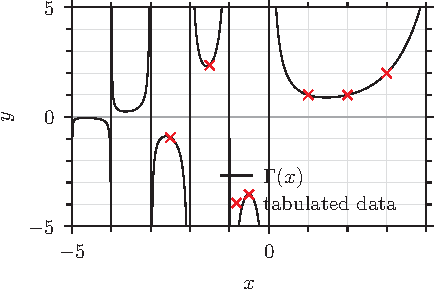
\includegraphics{gamma_pyx.pdf}
\end{figure}

\begin{figure}[b]
% GNUPLOT: LaTeX picture
\setlength{\unitlength}{0.240900pt}
\ifx\plotpoint\undefined\newsavebox{\plotpoint}\fi
\sbox{\plotpoint}{\rule[-0.200pt]{0.400pt}{0.400pt}}%
\begin{picture}(900,540)(0,0)
\sbox{\plotpoint}{\rule[-0.200pt]{0.400pt}{0.400pt}}%
\put(151.0,186.0){\rule[-0.200pt]{83.833pt}{0.400pt}}
\put(799.0,186.0){\rule[-0.200pt]{4.818pt}{0.400pt}}
\put(131.0,186.0){\rule[-0.200pt]{4.818pt}{0.400pt}}
\put(111,186){\makebox(0,0)[r]{$-4$}}
\put(819.0,186.0){\rule[-0.200pt]{4.818pt}{0.400pt}}
\put(151.0,255.0){\rule[-0.200pt]{160.921pt}{0.400pt}}
\put(131.0,255.0){\rule[-0.200pt]{4.818pt}{0.400pt}}
\put(111,255){\makebox(0,0)[r]{$-2$}}
\put(819.0,255.0){\rule[-0.200pt]{4.818pt}{0.400pt}}
\put(151.0,325.0){\rule[-0.200pt]{160.921pt}{0.400pt}}
\put(131.0,325.0){\rule[-0.200pt]{4.818pt}{0.400pt}}
\put(111,325){\makebox(0,0)[r]{$0$}}
\put(819.0,325.0){\rule[-0.200pt]{4.818pt}{0.400pt}}
\put(151.0,394.0){\rule[-0.200pt]{160.921pt}{0.400pt}}
\put(131.0,394.0){\rule[-0.200pt]{4.818pt}{0.400pt}}
\put(111,394){\makebox(0,0)[r]{$2$}}
\put(819.0,394.0){\rule[-0.200pt]{4.818pt}{0.400pt}}
\put(151.0,463.0){\rule[-0.200pt]{160.921pt}{0.400pt}}
\put(131.0,463.0){\rule[-0.200pt]{4.818pt}{0.400pt}}
\put(111,463){\makebox(0,0)[r]{$4$}}
\put(819.0,463.0){\rule[-0.200pt]{4.818pt}{0.400pt}}
\put(151.0,151.0){\rule[-0.200pt]{0.400pt}{83.592pt}}
\put(151.0,131.0){\rule[-0.200pt]{0.400pt}{4.818pt}}
\put(151,90){\makebox(0,0){$-5$}}
\put(151.0,498.0){\rule[-0.200pt]{0.400pt}{4.818pt}}
\put(218.0,151.0){\rule[-0.200pt]{0.400pt}{83.592pt}}
\put(218.0,131.0){\rule[-0.200pt]{0.400pt}{4.818pt}}
\put(218,90){\makebox(0,0){$-4$}}
\put(218.0,498.0){\rule[-0.200pt]{0.400pt}{4.818pt}}
\put(285.0,151.0){\rule[-0.200pt]{0.400pt}{83.592pt}}
\put(285.0,131.0){\rule[-0.200pt]{0.400pt}{4.818pt}}
\put(285,90){\makebox(0,0){$-3$}}
\put(285.0,498.0){\rule[-0.200pt]{0.400pt}{4.818pt}}
\put(351.0,151.0){\rule[-0.200pt]{0.400pt}{83.592pt}}
\put(351.0,131.0){\rule[-0.200pt]{0.400pt}{4.818pt}}
\put(351,90){\makebox(0,0){$-2$}}
\put(351.0,498.0){\rule[-0.200pt]{0.400pt}{4.818pt}}
\put(418.0,151.0){\rule[-0.200pt]{0.400pt}{83.592pt}}
\put(418.0,131.0){\rule[-0.200pt]{0.400pt}{4.818pt}}
\put(418,90){\makebox(0,0){$-1$}}
\put(418.0,498.0){\rule[-0.200pt]{0.400pt}{4.818pt}}
\put(485.0,151.0){\rule[-0.200pt]{0.400pt}{83.592pt}}
\put(485.0,131.0){\rule[-0.200pt]{0.400pt}{4.818pt}}
\put(485,90){\makebox(0,0){$0$}}
\put(485.0,498.0){\rule[-0.200pt]{0.400pt}{4.818pt}}
\put(552.0,151.0){\rule[-0.200pt]{0.400pt}{4.818pt}}
\put(552.0,253.0){\rule[-0.200pt]{0.400pt}{59.020pt}}
\put(552.0,131.0){\rule[-0.200pt]{0.400pt}{4.818pt}}
\put(552,90){\makebox(0,0){$1$}}
\put(552.0,498.0){\rule[-0.200pt]{0.400pt}{4.818pt}}
\put(619.0,151.0){\rule[-0.200pt]{0.400pt}{4.818pt}}
\put(619.0,253.0){\rule[-0.200pt]{0.400pt}{59.020pt}}
\put(619.0,131.0){\rule[-0.200pt]{0.400pt}{4.818pt}}
\put(619,90){\makebox(0,0){$2$}}
\put(619.0,498.0){\rule[-0.200pt]{0.400pt}{4.818pt}}
\put(685.0,151.0){\rule[-0.200pt]{0.400pt}{4.818pt}}
\put(685.0,253.0){\rule[-0.200pt]{0.400pt}{59.020pt}}
\put(685.0,131.0){\rule[-0.200pt]{0.400pt}{4.818pt}}
\put(685,90){\makebox(0,0){$3$}}
\put(685.0,498.0){\rule[-0.200pt]{0.400pt}{4.818pt}}
\put(752.0,151.0){\rule[-0.200pt]{0.400pt}{4.818pt}}
\put(752.0,253.0){\rule[-0.200pt]{0.400pt}{59.020pt}}
\put(752.0,131.0){\rule[-0.200pt]{0.400pt}{4.818pt}}
\put(752,90){\makebox(0,0){$4$}}
\put(752.0,498.0){\rule[-0.200pt]{0.400pt}{4.818pt}}
\put(819.0,151.0){\rule[-0.200pt]{0.400pt}{83.592pt}}
\put(819.0,131.0){\rule[-0.200pt]{0.400pt}{4.818pt}}
\put(819,90){\makebox(0,0){$5$}}
\put(819.0,498.0){\rule[-0.200pt]{0.400pt}{4.818pt}}
\put(151.0,151.0){\rule[-0.200pt]{0.400pt}{83.592pt}}
\put(151.0,151.0){\rule[-0.200pt]{160.921pt}{0.400pt}}
\put(819.0,151.0){\rule[-0.200pt]{0.400pt}{83.592pt}}
\put(151.0,498.0){\rule[-0.200pt]{160.921pt}{0.400pt}}
\put(36,324){\makebox(0,0){$y$}}
\put(485,29){\makebox(0,0){$x$}}
\put(659,232){\makebox(0,0)[r]{$Gamma(x)$}}
\put(679.0,232.0){\rule[-0.200pt]{24.090pt}{0.400pt}}
\put(152,287){\usebox{\plotpoint}}
\put(151.67,287){\rule{0.400pt}{6.023pt}}
\multiput(151.17,287.00)(1.000,12.500){2}{\rule{0.400pt}{3.011pt}}
\put(152.67,312){\rule{0.400pt}{1.204pt}}
\multiput(152.17,312.00)(1.000,2.500){2}{\rule{0.400pt}{0.602pt}}
\put(153.67,317){\rule{0.400pt}{0.482pt}}
\multiput(153.17,317.00)(1.000,1.000){2}{\rule{0.400pt}{0.241pt}}
\put(155,318.67){\rule{0.241pt}{0.400pt}}
\multiput(155.00,318.17)(0.500,1.000){2}{\rule{0.120pt}{0.400pt}}
\put(156,319.67){\rule{0.241pt}{0.400pt}}
\multiput(156.00,319.17)(0.500,1.000){2}{\rule{0.120pt}{0.400pt}}
\put(159,320.67){\rule{0.241pt}{0.400pt}}
\multiput(159.00,320.17)(0.500,1.000){2}{\rule{0.120pt}{0.400pt}}
\put(157.0,321.0){\rule[-0.200pt]{0.482pt}{0.400pt}}
\put(166,321.67){\rule{0.241pt}{0.400pt}}
\multiput(166.00,321.17)(0.500,1.000){2}{\rule{0.120pt}{0.400pt}}
\put(160.0,322.0){\rule[-0.200pt]{1.445pt}{0.400pt}}
\put(182,321.67){\rule{0.241pt}{0.400pt}}
\multiput(182.00,322.17)(0.500,-1.000){2}{\rule{0.120pt}{0.400pt}}
\put(167.0,323.0){\rule[-0.200pt]{3.613pt}{0.400pt}}
\put(194,320.67){\rule{0.241pt}{0.400pt}}
\multiput(194.00,321.17)(0.500,-1.000){2}{\rule{0.120pt}{0.400pt}}
\put(183.0,322.0){\rule[-0.200pt]{2.650pt}{0.400pt}}
\put(200,319.67){\rule{0.241pt}{0.400pt}}
\multiput(200.00,320.17)(0.500,-1.000){2}{\rule{0.120pt}{0.400pt}}
\put(195.0,321.0){\rule[-0.200pt]{1.204pt}{0.400pt}}
\put(203,318.67){\rule{0.241pt}{0.400pt}}
\multiput(203.00,319.17)(0.500,-1.000){2}{\rule{0.120pt}{0.400pt}}
\put(201.0,320.0){\rule[-0.200pt]{0.482pt}{0.400pt}}
\put(205,317.67){\rule{0.241pt}{0.400pt}}
\multiput(205.00,318.17)(0.500,-1.000){2}{\rule{0.120pt}{0.400pt}}
\put(206,316.67){\rule{0.241pt}{0.400pt}}
\multiput(206.00,317.17)(0.500,-1.000){2}{\rule{0.120pt}{0.400pt}}
\put(207,315.67){\rule{0.241pt}{0.400pt}}
\multiput(207.00,316.17)(0.500,-1.000){2}{\rule{0.120pt}{0.400pt}}
\put(208,314.67){\rule{0.241pt}{0.400pt}}
\multiput(208.00,315.17)(0.500,-1.000){2}{\rule{0.120pt}{0.400pt}}
\put(209,313.67){\rule{0.241pt}{0.400pt}}
\multiput(209.00,314.17)(0.500,-1.000){2}{\rule{0.120pt}{0.400pt}}
\put(209.67,312){\rule{0.400pt}{0.482pt}}
\multiput(209.17,313.00)(1.000,-1.000){2}{\rule{0.400pt}{0.241pt}}
\put(210.67,310){\rule{0.400pt}{0.482pt}}
\multiput(210.17,311.00)(1.000,-1.000){2}{\rule{0.400pt}{0.241pt}}
\put(211.67,306){\rule{0.400pt}{0.964pt}}
\multiput(211.17,308.00)(1.000,-2.000){2}{\rule{0.400pt}{0.482pt}}
\put(212.67,300){\rule{0.400pt}{1.445pt}}
\multiput(212.17,303.00)(1.000,-3.000){2}{\rule{0.400pt}{0.723pt}}
\put(213.67,290){\rule{0.400pt}{2.409pt}}
\multiput(213.17,295.00)(1.000,-5.000){2}{\rule{0.400pt}{1.204pt}}
\put(214.67,265){\rule{0.400pt}{6.023pt}}
\multiput(214.17,277.50)(1.000,-12.500){2}{\rule{0.400pt}{3.011pt}}
\put(204.0,319.0){\usebox{\plotpoint}}
\put(217.67,388){\rule{0.400pt}{26.499pt}}
\multiput(217.17,443.00)(1.000,-55.000){2}{\rule{0.400pt}{13.249pt}}
\put(218.67,364){\rule{0.400pt}{5.782pt}}
\multiput(218.17,376.00)(1.000,-12.000){2}{\rule{0.400pt}{2.891pt}}
\put(219.67,353){\rule{0.400pt}{2.650pt}}
\multiput(219.17,358.50)(1.000,-5.500){2}{\rule{0.400pt}{1.325pt}}
\put(220.67,348){\rule{0.400pt}{1.204pt}}
\multiput(220.17,350.50)(1.000,-2.500){2}{\rule{0.400pt}{0.602pt}}
\put(222.17,344){\rule{0.400pt}{0.900pt}}
\multiput(221.17,346.13)(2.000,-2.132){2}{\rule{0.400pt}{0.450pt}}
\put(223.67,341){\rule{0.400pt}{0.723pt}}
\multiput(223.17,342.50)(1.000,-1.500){2}{\rule{0.400pt}{0.361pt}}
\put(225,339.67){\rule{0.241pt}{0.400pt}}
\multiput(225.00,340.17)(0.500,-1.000){2}{\rule{0.120pt}{0.400pt}}
\put(225.67,338){\rule{0.400pt}{0.482pt}}
\multiput(225.17,339.00)(1.000,-1.000){2}{\rule{0.400pt}{0.241pt}}
\put(227,336.67){\rule{0.241pt}{0.400pt}}
\multiput(227.00,337.17)(0.500,-1.000){2}{\rule{0.120pt}{0.400pt}}
\put(228,335.67){\rule{0.241pt}{0.400pt}}
\multiput(228.00,336.17)(0.500,-1.000){2}{\rule{0.120pt}{0.400pt}}
\put(216.0,151.0){\rule[-0.200pt]{0.400pt}{27.463pt}}
\put(230,334.67){\rule{0.241pt}{0.400pt}}
\multiput(230.00,335.17)(0.500,-1.000){2}{\rule{0.120pt}{0.400pt}}
\put(229.0,336.0){\usebox{\plotpoint}}
\put(232,333.67){\rule{0.241pt}{0.400pt}}
\multiput(232.00,334.17)(0.500,-1.000){2}{\rule{0.120pt}{0.400pt}}
\put(231.0,335.0){\usebox{\plotpoint}}
\put(235,332.67){\rule{0.241pt}{0.400pt}}
\multiput(235.00,333.17)(0.500,-1.000){2}{\rule{0.120pt}{0.400pt}}
\put(233.0,334.0){\rule[-0.200pt]{0.482pt}{0.400pt}}
\put(249,332.67){\rule{0.241pt}{0.400pt}}
\multiput(249.00,332.17)(0.500,1.000){2}{\rule{0.120pt}{0.400pt}}
\put(236.0,333.0){\rule[-0.200pt]{3.132pt}{0.400pt}}
\put(254,333.67){\rule{0.241pt}{0.400pt}}
\multiput(254.00,333.17)(0.500,1.000){2}{\rule{0.120pt}{0.400pt}}
\put(250.0,334.0){\rule[-0.200pt]{0.964pt}{0.400pt}}
\put(257,334.67){\rule{0.241pt}{0.400pt}}
\multiput(257.00,334.17)(0.500,1.000){2}{\rule{0.120pt}{0.400pt}}
\put(255.0,335.0){\rule[-0.200pt]{0.482pt}{0.400pt}}
\put(259,335.67){\rule{0.241pt}{0.400pt}}
\multiput(259.00,335.17)(0.500,1.000){2}{\rule{0.120pt}{0.400pt}}
\put(258.0,336.0){\usebox{\plotpoint}}
\put(261,336.67){\rule{0.241pt}{0.400pt}}
\multiput(261.00,336.17)(0.500,1.000){2}{\rule{0.120pt}{0.400pt}}
\put(262,337.67){\rule{0.241pt}{0.400pt}}
\multiput(262.00,337.17)(0.500,1.000){2}{\rule{0.120pt}{0.400pt}}
\put(260.0,337.0){\usebox{\plotpoint}}
\put(264,338.67){\rule{0.241pt}{0.400pt}}
\multiput(264.00,338.17)(0.500,1.000){2}{\rule{0.120pt}{0.400pt}}
\put(265,339.67){\rule{0.241pt}{0.400pt}}
\multiput(265.00,339.17)(0.500,1.000){2}{\rule{0.120pt}{0.400pt}}
\put(266,340.67){\rule{0.241pt}{0.400pt}}
\multiput(266.00,340.17)(0.500,1.000){2}{\rule{0.120pt}{0.400pt}}
\put(266.67,342){\rule{0.400pt}{0.482pt}}
\multiput(266.17,342.00)(1.000,1.000){2}{\rule{0.400pt}{0.241pt}}
\put(268,343.67){\rule{0.241pt}{0.400pt}}
\multiput(268.00,343.17)(0.500,1.000){2}{\rule{0.120pt}{0.400pt}}
\put(269,345.17){\rule{0.482pt}{0.400pt}}
\multiput(269.00,344.17)(1.000,2.000){2}{\rule{0.241pt}{0.400pt}}
\put(270.67,347){\rule{0.400pt}{0.482pt}}
\multiput(270.17,347.00)(1.000,1.000){2}{\rule{0.400pt}{0.241pt}}
\put(271.67,349){\rule{0.400pt}{0.482pt}}
\multiput(271.17,349.00)(1.000,1.000){2}{\rule{0.400pt}{0.241pt}}
\put(272.67,351){\rule{0.400pt}{0.723pt}}
\multiput(272.17,351.00)(1.000,1.500){2}{\rule{0.400pt}{0.361pt}}
\put(273.67,354){\rule{0.400pt}{0.964pt}}
\multiput(273.17,354.00)(1.000,2.000){2}{\rule{0.400pt}{0.482pt}}
\put(274.67,358){\rule{0.400pt}{0.964pt}}
\multiput(274.17,358.00)(1.000,2.000){2}{\rule{0.400pt}{0.482pt}}
\put(275.67,362){\rule{0.400pt}{1.445pt}}
\multiput(275.17,362.00)(1.000,3.000){2}{\rule{0.400pt}{0.723pt}}
\put(276.67,368){\rule{0.400pt}{1.686pt}}
\multiput(276.17,368.00)(1.000,3.500){2}{\rule{0.400pt}{0.843pt}}
\put(277.67,375){\rule{0.400pt}{2.650pt}}
\multiput(277.17,375.00)(1.000,5.500){2}{\rule{0.400pt}{1.325pt}}
\put(278.67,386){\rule{0.400pt}{3.373pt}}
\multiput(278.17,386.00)(1.000,7.000){2}{\rule{0.400pt}{1.686pt}}
\put(279.67,400){\rule{0.400pt}{5.782pt}}
\multiput(279.17,400.00)(1.000,12.000){2}{\rule{0.400pt}{2.891pt}}
\put(280.67,424){\rule{0.400pt}{10.118pt}}
\multiput(280.17,424.00)(1.000,21.000){2}{\rule{0.400pt}{5.059pt}}
\put(263.0,339.0){\usebox{\plotpoint}}
\put(285.67,151){\rule{0.400pt}{4.336pt}}
\multiput(285.17,151.00)(1.000,9.000){2}{\rule{0.400pt}{2.168pt}}
\put(286.67,169){\rule{0.400pt}{10.118pt}}
\multiput(286.17,169.00)(1.000,21.000){2}{\rule{0.400pt}{5.059pt}}
\put(287.67,211){\rule{0.400pt}{5.541pt}}
\multiput(287.17,211.00)(1.000,11.500){2}{\rule{0.400pt}{2.770pt}}
\put(288.67,234){\rule{0.400pt}{3.614pt}}
\multiput(288.17,234.00)(1.000,7.500){2}{\rule{0.400pt}{1.807pt}}
\put(289.67,249){\rule{0.400pt}{2.409pt}}
\multiput(289.17,249.00)(1.000,5.000){2}{\rule{0.400pt}{1.204pt}}
\put(290.67,259){\rule{0.400pt}{1.686pt}}
\multiput(290.17,259.00)(1.000,3.500){2}{\rule{0.400pt}{0.843pt}}
\put(291.67,266){\rule{0.400pt}{1.445pt}}
\multiput(291.17,266.00)(1.000,3.000){2}{\rule{0.400pt}{0.723pt}}
\put(293.17,272){\rule{0.400pt}{0.900pt}}
\multiput(292.17,272.00)(2.000,2.132){2}{\rule{0.400pt}{0.450pt}}
\put(294.67,276){\rule{0.400pt}{0.723pt}}
\multiput(294.17,276.00)(1.000,1.500){2}{\rule{0.400pt}{0.361pt}}
\put(295.67,279){\rule{0.400pt}{0.723pt}}
\multiput(295.17,279.00)(1.000,1.500){2}{\rule{0.400pt}{0.361pt}}
\put(296.67,282){\rule{0.400pt}{0.482pt}}
\multiput(296.17,282.00)(1.000,1.000){2}{\rule{0.400pt}{0.241pt}}
\put(297.67,284){\rule{0.400pt}{0.482pt}}
\multiput(297.17,284.00)(1.000,1.000){2}{\rule{0.400pt}{0.241pt}}
\put(298.67,286){\rule{0.400pt}{0.482pt}}
\multiput(298.17,286.00)(1.000,1.000){2}{\rule{0.400pt}{0.241pt}}
\put(300,287.67){\rule{0.241pt}{0.400pt}}
\multiput(300.00,287.17)(0.500,1.000){2}{\rule{0.120pt}{0.400pt}}
\put(301,288.67){\rule{0.241pt}{0.400pt}}
\multiput(301.00,288.17)(0.500,1.000){2}{\rule{0.120pt}{0.400pt}}
\put(302,289.67){\rule{0.241pt}{0.400pt}}
\multiput(302.00,289.17)(0.500,1.000){2}{\rule{0.120pt}{0.400pt}}
\put(303,290.67){\rule{0.241pt}{0.400pt}}
\multiput(303.00,290.17)(0.500,1.000){2}{\rule{0.120pt}{0.400pt}}
\put(282.0,466.0){\rule[-0.200pt]{0.400pt}{7.709pt}}
\put(305,291.67){\rule{0.241pt}{0.400pt}}
\multiput(305.00,291.17)(0.500,1.000){2}{\rule{0.120pt}{0.400pt}}
\put(304.0,292.0){\usebox{\plotpoint}}
\put(308,292.67){\rule{0.241pt}{0.400pt}}
\multiput(308.00,292.17)(0.500,1.000){2}{\rule{0.120pt}{0.400pt}}
\put(306.0,293.0){\rule[-0.200pt]{0.482pt}{0.400pt}}
\put(312,292.67){\rule{0.241pt}{0.400pt}}
\multiput(312.00,293.17)(0.500,-1.000){2}{\rule{0.120pt}{0.400pt}}
\put(309.0,294.0){\rule[-0.200pt]{0.723pt}{0.400pt}}
\put(315,291.67){\rule{0.241pt}{0.400pt}}
\multiput(315.00,292.17)(0.500,-1.000){2}{\rule{0.120pt}{0.400pt}}
\put(313.0,293.0){\rule[-0.200pt]{0.482pt}{0.400pt}}
\put(317,290.67){\rule{0.482pt}{0.400pt}}
\multiput(317.00,291.17)(1.000,-1.000){2}{\rule{0.241pt}{0.400pt}}
\put(316.0,292.0){\usebox{\plotpoint}}
\put(320,289.67){\rule{0.241pt}{0.400pt}}
\multiput(320.00,290.17)(0.500,-1.000){2}{\rule{0.120pt}{0.400pt}}
\put(321,288.67){\rule{0.241pt}{0.400pt}}
\multiput(321.00,289.17)(0.500,-1.000){2}{\rule{0.120pt}{0.400pt}}
\put(322,287.67){\rule{0.241pt}{0.400pt}}
\multiput(322.00,288.17)(0.500,-1.000){2}{\rule{0.120pt}{0.400pt}}
\put(323,286.67){\rule{0.241pt}{0.400pt}}
\multiput(323.00,287.17)(0.500,-1.000){2}{\rule{0.120pt}{0.400pt}}
\put(324,285.67){\rule{0.241pt}{0.400pt}}
\multiput(324.00,286.17)(0.500,-1.000){2}{\rule{0.120pt}{0.400pt}}
\put(325,284.67){\rule{0.241pt}{0.400pt}}
\multiput(325.00,285.17)(0.500,-1.000){2}{\rule{0.120pt}{0.400pt}}
\put(325.67,283){\rule{0.400pt}{0.482pt}}
\multiput(325.17,284.00)(1.000,-1.000){2}{\rule{0.400pt}{0.241pt}}
\put(326.67,281){\rule{0.400pt}{0.482pt}}
\multiput(326.17,282.00)(1.000,-1.000){2}{\rule{0.400pt}{0.241pt}}
\put(328,279.67){\rule{0.241pt}{0.400pt}}
\multiput(328.00,280.17)(0.500,-1.000){2}{\rule{0.120pt}{0.400pt}}
\put(328.67,277){\rule{0.400pt}{0.723pt}}
\multiput(328.17,278.50)(1.000,-1.500){2}{\rule{0.400pt}{0.361pt}}
\put(329.67,275){\rule{0.400pt}{0.482pt}}
\multiput(329.17,276.00)(1.000,-1.000){2}{\rule{0.400pt}{0.241pt}}
\put(330.67,272){\rule{0.400pt}{0.723pt}}
\multiput(330.17,273.50)(1.000,-1.500){2}{\rule{0.400pt}{0.361pt}}
\put(331.67,269){\rule{0.400pt}{0.723pt}}
\multiput(331.17,270.50)(1.000,-1.500){2}{\rule{0.400pt}{0.361pt}}
\put(332.67,266){\rule{0.400pt}{0.723pt}}
\multiput(332.17,267.50)(1.000,-1.500){2}{\rule{0.400pt}{0.361pt}}
\put(333.67,262){\rule{0.400pt}{0.964pt}}
\multiput(333.17,264.00)(1.000,-2.000){2}{\rule{0.400pt}{0.482pt}}
\put(334.67,257){\rule{0.400pt}{1.204pt}}
\multiput(334.17,259.50)(1.000,-2.500){2}{\rule{0.400pt}{0.602pt}}
\put(335.67,252){\rule{0.400pt}{1.204pt}}
\multiput(335.17,254.50)(1.000,-2.500){2}{\rule{0.400pt}{0.602pt}}
\put(336.67,246){\rule{0.400pt}{1.445pt}}
\multiput(336.17,249.00)(1.000,-3.000){2}{\rule{0.400pt}{0.723pt}}
\put(337.67,239){\rule{0.400pt}{1.686pt}}
\multiput(337.17,242.50)(1.000,-3.500){2}{\rule{0.400pt}{0.843pt}}
\put(338.67,230){\rule{0.400pt}{2.168pt}}
\multiput(338.17,234.50)(1.000,-4.500){2}{\rule{0.400pt}{1.084pt}}
\put(339.67,219){\rule{0.400pt}{2.650pt}}
\multiput(339.17,224.50)(1.000,-5.500){2}{\rule{0.400pt}{1.325pt}}
\put(341.17,206){\rule{0.400pt}{2.700pt}}
\multiput(340.17,213.40)(2.000,-7.396){2}{\rule{0.400pt}{1.350pt}}
\put(342.67,189){\rule{0.400pt}{4.095pt}}
\multiput(342.17,197.50)(1.000,-8.500){2}{\rule{0.400pt}{2.048pt}}
\put(343.67,167){\rule{0.400pt}{5.300pt}}
\multiput(343.17,178.00)(1.000,-11.000){2}{\rule{0.400pt}{2.650pt}}
\put(319.0,291.0){\usebox{\plotpoint}}
\put(357.67,493){\rule{0.400pt}{1.204pt}}
\multiput(357.17,495.50)(1.000,-2.500){2}{\rule{0.400pt}{0.602pt}}
\put(358.67,476){\rule{0.400pt}{4.095pt}}
\multiput(358.17,484.50)(1.000,-8.500){2}{\rule{0.400pt}{2.048pt}}
\put(359.67,463){\rule{0.400pt}{3.132pt}}
\multiput(359.17,469.50)(1.000,-6.500){2}{\rule{0.400pt}{1.566pt}}
\put(360.67,452){\rule{0.400pt}{2.650pt}}
\multiput(360.17,457.50)(1.000,-5.500){2}{\rule{0.400pt}{1.325pt}}
\put(361.67,444){\rule{0.400pt}{1.927pt}}
\multiput(361.17,448.00)(1.000,-4.000){2}{\rule{0.400pt}{0.964pt}}
\put(362.67,437){\rule{0.400pt}{1.686pt}}
\multiput(362.17,440.50)(1.000,-3.500){2}{\rule{0.400pt}{0.843pt}}
\put(363.67,431){\rule{0.400pt}{1.445pt}}
\multiput(363.17,434.00)(1.000,-3.000){2}{\rule{0.400pt}{0.723pt}}
\put(365.17,426){\rule{0.400pt}{1.100pt}}
\multiput(364.17,428.72)(2.000,-2.717){2}{\rule{0.400pt}{0.550pt}}
\put(366.67,422){\rule{0.400pt}{0.964pt}}
\multiput(366.17,424.00)(1.000,-2.000){2}{\rule{0.400pt}{0.482pt}}
\put(367.67,419){\rule{0.400pt}{0.723pt}}
\multiput(367.17,420.50)(1.000,-1.500){2}{\rule{0.400pt}{0.361pt}}
\put(368.67,416){\rule{0.400pt}{0.723pt}}
\multiput(368.17,417.50)(1.000,-1.500){2}{\rule{0.400pt}{0.361pt}}
\put(369.67,413){\rule{0.400pt}{0.723pt}}
\multiput(369.17,414.50)(1.000,-1.500){2}{\rule{0.400pt}{0.361pt}}
\put(370.67,411){\rule{0.400pt}{0.482pt}}
\multiput(370.17,412.00)(1.000,-1.000){2}{\rule{0.400pt}{0.241pt}}
\put(371.67,409){\rule{0.400pt}{0.482pt}}
\multiput(371.17,410.00)(1.000,-1.000){2}{\rule{0.400pt}{0.241pt}}
\put(373,407.67){\rule{0.241pt}{0.400pt}}
\multiput(373.00,408.17)(0.500,-1.000){2}{\rule{0.120pt}{0.400pt}}
\put(374,406.67){\rule{0.241pt}{0.400pt}}
\multiput(374.00,407.17)(0.500,-1.000){2}{\rule{0.120pt}{0.400pt}}
\put(375,405.67){\rule{0.241pt}{0.400pt}}
\multiput(375.00,406.17)(0.500,-1.000){2}{\rule{0.120pt}{0.400pt}}
\put(376,404.67){\rule{0.241pt}{0.400pt}}
\multiput(376.00,405.17)(0.500,-1.000){2}{\rule{0.120pt}{0.400pt}}
\put(345.0,151.0){\rule[-0.200pt]{0.400pt}{3.854pt}}
\put(378,403.67){\rule{0.241pt}{0.400pt}}
\multiput(378.00,404.17)(0.500,-1.000){2}{\rule{0.120pt}{0.400pt}}
\put(377.0,405.0){\usebox{\plotpoint}}
\put(380,403.67){\rule{0.241pt}{0.400pt}}
\multiput(380.00,403.17)(0.500,1.000){2}{\rule{0.120pt}{0.400pt}}
\put(379.0,404.0){\usebox{\plotpoint}}
\put(383,404.67){\rule{0.241pt}{0.400pt}}
\multiput(383.00,404.17)(0.500,1.000){2}{\rule{0.120pt}{0.400pt}}
\put(384,405.67){\rule{0.241pt}{0.400pt}}
\multiput(384.00,405.17)(0.500,1.000){2}{\rule{0.120pt}{0.400pt}}
\put(385,406.67){\rule{0.241pt}{0.400pt}}
\multiput(385.00,406.17)(0.500,1.000){2}{\rule{0.120pt}{0.400pt}}
\put(386,407.67){\rule{0.241pt}{0.400pt}}
\multiput(386.00,407.17)(0.500,1.000){2}{\rule{0.120pt}{0.400pt}}
\put(386.67,409){\rule{0.400pt}{0.482pt}}
\multiput(386.17,409.00)(1.000,1.000){2}{\rule{0.400pt}{0.241pt}}
\put(387.67,411){\rule{0.400pt}{0.482pt}}
\multiput(387.17,411.00)(1.000,1.000){2}{\rule{0.400pt}{0.241pt}}
\put(389,413.17){\rule{0.482pt}{0.400pt}}
\multiput(389.00,412.17)(1.000,2.000){2}{\rule{0.241pt}{0.400pt}}
\put(390.67,415){\rule{0.400pt}{0.482pt}}
\multiput(390.17,415.00)(1.000,1.000){2}{\rule{0.400pt}{0.241pt}}
\put(391.67,417){\rule{0.400pt}{0.723pt}}
\multiput(391.17,417.00)(1.000,1.500){2}{\rule{0.400pt}{0.361pt}}
\put(392.67,420){\rule{0.400pt}{0.723pt}}
\multiput(392.17,420.00)(1.000,1.500){2}{\rule{0.400pt}{0.361pt}}
\put(393.67,423){\rule{0.400pt}{0.723pt}}
\multiput(393.17,423.00)(1.000,1.500){2}{\rule{0.400pt}{0.361pt}}
\put(394.67,426){\rule{0.400pt}{0.964pt}}
\multiput(394.17,426.00)(1.000,2.000){2}{\rule{0.400pt}{0.482pt}}
\put(395.67,430){\rule{0.400pt}{0.964pt}}
\multiput(395.17,430.00)(1.000,2.000){2}{\rule{0.400pt}{0.482pt}}
\put(396.67,434){\rule{0.400pt}{0.964pt}}
\multiput(396.17,434.00)(1.000,2.000){2}{\rule{0.400pt}{0.482pt}}
\put(397.67,438){\rule{0.400pt}{1.445pt}}
\multiput(397.17,438.00)(1.000,3.000){2}{\rule{0.400pt}{0.723pt}}
\put(398.67,444){\rule{0.400pt}{1.445pt}}
\multiput(398.17,444.00)(1.000,3.000){2}{\rule{0.400pt}{0.723pt}}
\put(399.67,450){\rule{0.400pt}{1.686pt}}
\multiput(399.17,450.00)(1.000,3.500){2}{\rule{0.400pt}{0.843pt}}
\put(400.67,457){\rule{0.400pt}{1.927pt}}
\multiput(400.17,457.00)(1.000,4.000){2}{\rule{0.400pt}{0.964pt}}
\put(401.67,465){\rule{0.400pt}{2.168pt}}
\multiput(401.17,465.00)(1.000,4.500){2}{\rule{0.400pt}{1.084pt}}
\put(402.67,474){\rule{0.400pt}{2.409pt}}
\multiput(402.17,474.00)(1.000,5.000){2}{\rule{0.400pt}{1.204pt}}
\put(403.67,484){\rule{0.400pt}{3.132pt}}
\multiput(403.17,484.00)(1.000,6.500){2}{\rule{0.400pt}{1.566pt}}
\put(381.0,405.0){\rule[-0.200pt]{0.482pt}{0.400pt}}
\put(432.67,151){\rule{0.400pt}{0.482pt}}
\multiput(432.17,151.00)(1.000,1.000){2}{\rule{0.400pt}{0.241pt}}
\put(433.67,153){\rule{0.400pt}{1.686pt}}
\multiput(433.17,153.00)(1.000,3.500){2}{\rule{0.400pt}{0.843pt}}
\put(434.67,160){\rule{0.400pt}{1.686pt}}
\multiput(434.17,160.00)(1.000,3.500){2}{\rule{0.400pt}{0.843pt}}
\put(436.17,167){\rule{0.400pt}{1.300pt}}
\multiput(435.17,167.00)(2.000,3.302){2}{\rule{0.400pt}{0.650pt}}
\put(437.67,173){\rule{0.400pt}{1.204pt}}
\multiput(437.17,173.00)(1.000,2.500){2}{\rule{0.400pt}{0.602pt}}
\put(438.67,178){\rule{0.400pt}{0.964pt}}
\multiput(438.17,178.00)(1.000,2.000){2}{\rule{0.400pt}{0.482pt}}
\put(439.67,182){\rule{0.400pt}{0.964pt}}
\multiput(439.17,182.00)(1.000,2.000){2}{\rule{0.400pt}{0.482pt}}
\put(440.67,186){\rule{0.400pt}{0.723pt}}
\multiput(440.17,186.00)(1.000,1.500){2}{\rule{0.400pt}{0.361pt}}
\put(441.67,189){\rule{0.400pt}{0.723pt}}
\multiput(441.17,189.00)(1.000,1.500){2}{\rule{0.400pt}{0.361pt}}
\put(442.67,192){\rule{0.400pt}{0.482pt}}
\multiput(442.17,192.00)(1.000,1.000){2}{\rule{0.400pt}{0.241pt}}
\put(443.67,194){\rule{0.400pt}{0.482pt}}
\multiput(443.17,194.00)(1.000,1.000){2}{\rule{0.400pt}{0.241pt}}
\put(444.67,196){\rule{0.400pt}{0.482pt}}
\multiput(444.17,196.00)(1.000,1.000){2}{\rule{0.400pt}{0.241pt}}
\put(446,197.67){\rule{0.241pt}{0.400pt}}
\multiput(446.00,197.17)(0.500,1.000){2}{\rule{0.120pt}{0.400pt}}
\put(447,198.67){\rule{0.241pt}{0.400pt}}
\multiput(447.00,198.17)(0.500,1.000){2}{\rule{0.120pt}{0.400pt}}
\put(448,199.67){\rule{0.241pt}{0.400pt}}
\multiput(448.00,199.17)(0.500,1.000){2}{\rule{0.120pt}{0.400pt}}
\put(405.0,497.0){\usebox{\plotpoint}}
\put(453,199.67){\rule{0.241pt}{0.400pt}}
\multiput(453.00,200.17)(0.500,-1.000){2}{\rule{0.120pt}{0.400pt}}
\put(449.0,201.0){\rule[-0.200pt]{0.964pt}{0.400pt}}
\put(454.67,198){\rule{0.400pt}{0.482pt}}
\multiput(454.17,199.00)(1.000,-1.000){2}{\rule{0.400pt}{0.241pt}}
\put(456,196.67){\rule{0.241pt}{0.400pt}}
\multiput(456.00,197.17)(0.500,-1.000){2}{\rule{0.120pt}{0.400pt}}
\put(456.67,195){\rule{0.400pt}{0.482pt}}
\multiput(456.17,196.00)(1.000,-1.000){2}{\rule{0.400pt}{0.241pt}}
\put(457.67,193){\rule{0.400pt}{0.482pt}}
\multiput(457.17,194.00)(1.000,-1.000){2}{\rule{0.400pt}{0.241pt}}
\put(458.67,190){\rule{0.400pt}{0.723pt}}
\multiput(458.17,191.50)(1.000,-1.500){2}{\rule{0.400pt}{0.361pt}}
\put(460,188.17){\rule{0.482pt}{0.400pt}}
\multiput(460.00,189.17)(1.000,-2.000){2}{\rule{0.241pt}{0.400pt}}
\put(461.67,184){\rule{0.400pt}{0.964pt}}
\multiput(461.17,186.00)(1.000,-2.000){2}{\rule{0.400pt}{0.482pt}}
\put(462.67,180){\rule{0.400pt}{0.964pt}}
\multiput(462.17,182.00)(1.000,-2.000){2}{\rule{0.400pt}{0.482pt}}
\put(463.67,176){\rule{0.400pt}{0.964pt}}
\multiput(463.17,178.00)(1.000,-2.000){2}{\rule{0.400pt}{0.482pt}}
\put(464.67,171){\rule{0.400pt}{1.204pt}}
\multiput(464.17,173.50)(1.000,-2.500){2}{\rule{0.400pt}{0.602pt}}
\put(465.67,165){\rule{0.400pt}{1.445pt}}
\multiput(465.17,168.00)(1.000,-3.000){2}{\rule{0.400pt}{0.723pt}}
\put(466.67,158){\rule{0.400pt}{1.686pt}}
\multiput(466.17,161.50)(1.000,-3.500){2}{\rule{0.400pt}{0.843pt}}
\put(454.0,200.0){\usebox{\plotpoint}}
\put(496.67,488){\rule{0.400pt}{2.409pt}}
\multiput(496.17,493.00)(1.000,-5.000){2}{\rule{0.400pt}{1.204pt}}
\put(497.67,475){\rule{0.400pt}{3.132pt}}
\multiput(497.17,481.50)(1.000,-6.500){2}{\rule{0.400pt}{1.566pt}}
\put(498.67,464){\rule{0.400pt}{2.650pt}}
\multiput(498.17,469.50)(1.000,-5.500){2}{\rule{0.400pt}{1.325pt}}
\put(499.67,455){\rule{0.400pt}{2.168pt}}
\multiput(499.17,459.50)(1.000,-4.500){2}{\rule{0.400pt}{1.084pt}}
\put(500.67,446){\rule{0.400pt}{2.168pt}}
\multiput(500.17,450.50)(1.000,-4.500){2}{\rule{0.400pt}{1.084pt}}
\put(501.67,439){\rule{0.400pt}{1.686pt}}
\multiput(501.17,442.50)(1.000,-3.500){2}{\rule{0.400pt}{0.843pt}}
\put(502.67,432){\rule{0.400pt}{1.686pt}}
\multiput(502.17,435.50)(1.000,-3.500){2}{\rule{0.400pt}{0.843pt}}
\put(503.67,427){\rule{0.400pt}{1.204pt}}
\multiput(503.17,429.50)(1.000,-2.500){2}{\rule{0.400pt}{0.602pt}}
\put(504.67,421){\rule{0.400pt}{1.445pt}}
\multiput(504.17,424.00)(1.000,-3.000){2}{\rule{0.400pt}{0.723pt}}
\put(505.67,417){\rule{0.400pt}{0.964pt}}
\multiput(505.17,419.00)(1.000,-2.000){2}{\rule{0.400pt}{0.482pt}}
\put(506.67,412){\rule{0.400pt}{1.204pt}}
\multiput(506.17,414.50)(1.000,-2.500){2}{\rule{0.400pt}{0.602pt}}
\put(508.17,409){\rule{0.400pt}{0.700pt}}
\multiput(507.17,410.55)(2.000,-1.547){2}{\rule{0.400pt}{0.350pt}}
\put(509.67,405){\rule{0.400pt}{0.964pt}}
\multiput(509.17,407.00)(1.000,-2.000){2}{\rule{0.400pt}{0.482pt}}
\put(510.67,402){\rule{0.400pt}{0.723pt}}
\multiput(510.17,403.50)(1.000,-1.500){2}{\rule{0.400pt}{0.361pt}}
\put(511.67,399){\rule{0.400pt}{0.723pt}}
\multiput(511.17,400.50)(1.000,-1.500){2}{\rule{0.400pt}{0.361pt}}
\put(512.67,396){\rule{0.400pt}{0.723pt}}
\multiput(512.17,397.50)(1.000,-1.500){2}{\rule{0.400pt}{0.361pt}}
\put(513.67,394){\rule{0.400pt}{0.482pt}}
\multiput(513.17,395.00)(1.000,-1.000){2}{\rule{0.400pt}{0.241pt}}
\put(514.67,391){\rule{0.400pt}{0.723pt}}
\multiput(514.17,392.50)(1.000,-1.500){2}{\rule{0.400pt}{0.361pt}}
\put(515.67,389){\rule{0.400pt}{0.482pt}}
\multiput(515.17,390.00)(1.000,-1.000){2}{\rule{0.400pt}{0.241pt}}
\put(516.67,387){\rule{0.400pt}{0.482pt}}
\multiput(516.17,388.00)(1.000,-1.000){2}{\rule{0.400pt}{0.241pt}}
\put(517.67,385){\rule{0.400pt}{0.482pt}}
\multiput(517.17,386.00)(1.000,-1.000){2}{\rule{0.400pt}{0.241pt}}
\put(518.67,383){\rule{0.400pt}{0.482pt}}
\multiput(518.17,384.00)(1.000,-1.000){2}{\rule{0.400pt}{0.241pt}}
\put(520,381.67){\rule{0.241pt}{0.400pt}}
\multiput(520.00,382.17)(0.500,-1.000){2}{\rule{0.120pt}{0.400pt}}
\put(520.67,380){\rule{0.400pt}{0.482pt}}
\multiput(520.17,381.00)(1.000,-1.000){2}{\rule{0.400pt}{0.241pt}}
\put(522,378.67){\rule{0.241pt}{0.400pt}}
\multiput(522.00,379.17)(0.500,-1.000){2}{\rule{0.120pt}{0.400pt}}
\put(522.67,377){\rule{0.400pt}{0.482pt}}
\multiput(522.17,378.00)(1.000,-1.000){2}{\rule{0.400pt}{0.241pt}}
\put(524,375.67){\rule{0.241pt}{0.400pt}}
\multiput(524.00,376.17)(0.500,-1.000){2}{\rule{0.120pt}{0.400pt}}
\put(525,374.67){\rule{0.241pt}{0.400pt}}
\multiput(525.00,375.17)(0.500,-1.000){2}{\rule{0.120pt}{0.400pt}}
\put(526,373.67){\rule{0.241pt}{0.400pt}}
\multiput(526.00,374.17)(0.500,-1.000){2}{\rule{0.120pt}{0.400pt}}
\put(527,372.67){\rule{0.241pt}{0.400pt}}
\multiput(527.00,373.17)(0.500,-1.000){2}{\rule{0.120pt}{0.400pt}}
\put(528,371.67){\rule{0.241pt}{0.400pt}}
\multiput(528.00,372.17)(0.500,-1.000){2}{\rule{0.120pt}{0.400pt}}
\put(529,370.67){\rule{0.241pt}{0.400pt}}
\multiput(529.00,371.17)(0.500,-1.000){2}{\rule{0.120pt}{0.400pt}}
\put(530,369.67){\rule{0.241pt}{0.400pt}}
\multiput(530.00,370.17)(0.500,-1.000){2}{\rule{0.120pt}{0.400pt}}
\put(531,368.67){\rule{0.241pt}{0.400pt}}
\multiput(531.00,369.17)(0.500,-1.000){2}{\rule{0.120pt}{0.400pt}}
\put(532,367.67){\rule{0.482pt}{0.400pt}}
\multiput(532.00,368.17)(1.000,-1.000){2}{\rule{0.241pt}{0.400pt}}
\put(534,366.67){\rule{0.241pt}{0.400pt}}
\multiput(534.00,367.17)(0.500,-1.000){2}{\rule{0.120pt}{0.400pt}}
\put(468.0,151.0){\rule[-0.200pt]{0.400pt}{1.686pt}}
\put(536,365.67){\rule{0.241pt}{0.400pt}}
\multiput(536.00,366.17)(0.500,-1.000){2}{\rule{0.120pt}{0.400pt}}
\put(537,364.67){\rule{0.241pt}{0.400pt}}
\multiput(537.00,365.17)(0.500,-1.000){2}{\rule{0.120pt}{0.400pt}}
\put(535.0,367.0){\usebox{\plotpoint}}
\put(539,363.67){\rule{0.241pt}{0.400pt}}
\multiput(539.00,364.17)(0.500,-1.000){2}{\rule{0.120pt}{0.400pt}}
\put(538.0,365.0){\usebox{\plotpoint}}
\put(541,362.67){\rule{0.241pt}{0.400pt}}
\multiput(541.00,363.17)(0.500,-1.000){2}{\rule{0.120pt}{0.400pt}}
\put(540.0,364.0){\usebox{\plotpoint}}
\put(543,361.67){\rule{0.241pt}{0.400pt}}
\multiput(543.00,362.17)(0.500,-1.000){2}{\rule{0.120pt}{0.400pt}}
\put(542.0,363.0){\usebox{\plotpoint}}
\put(545,360.67){\rule{0.241pt}{0.400pt}}
\multiput(545.00,361.17)(0.500,-1.000){2}{\rule{0.120pt}{0.400pt}}
\put(544.0,362.0){\usebox{\plotpoint}}
\put(547,359.67){\rule{0.241pt}{0.400pt}}
\multiput(547.00,360.17)(0.500,-1.000){2}{\rule{0.120pt}{0.400pt}}
\put(546.0,361.0){\usebox{\plotpoint}}
\put(550,358.67){\rule{0.241pt}{0.400pt}}
\multiput(550.00,359.17)(0.500,-1.000){2}{\rule{0.120pt}{0.400pt}}
\put(548.0,360.0){\rule[-0.200pt]{0.482pt}{0.400pt}}
\put(553,357.67){\rule{0.241pt}{0.400pt}}
\multiput(553.00,358.17)(0.500,-1.000){2}{\rule{0.120pt}{0.400pt}}
\put(551.0,359.0){\rule[-0.200pt]{0.482pt}{0.400pt}}
\put(558,356.67){\rule{0.241pt}{0.400pt}}
\multiput(558.00,357.17)(0.500,-1.000){2}{\rule{0.120pt}{0.400pt}}
\put(554.0,358.0){\rule[-0.200pt]{0.964pt}{0.400pt}}
\put(564,355.67){\rule{0.241pt}{0.400pt}}
\multiput(564.00,356.17)(0.500,-1.000){2}{\rule{0.120pt}{0.400pt}}
\put(559.0,357.0){\rule[-0.200pt]{1.204pt}{0.400pt}}
\put(573,354.67){\rule{0.241pt}{0.400pt}}
\multiput(573.00,355.17)(0.500,-1.000){2}{\rule{0.120pt}{0.400pt}}
\put(565.0,356.0){\rule[-0.200pt]{1.927pt}{0.400pt}}
\put(591,354.67){\rule{0.241pt}{0.400pt}}
\multiput(591.00,354.17)(0.500,1.000){2}{\rule{0.120pt}{0.400pt}}
\put(574.0,355.0){\rule[-0.200pt]{4.095pt}{0.400pt}}
\put(602,355.67){\rule{0.241pt}{0.400pt}}
\multiput(602.00,355.17)(0.500,1.000){2}{\rule{0.120pt}{0.400pt}}
\put(592.0,356.0){\rule[-0.200pt]{2.409pt}{0.400pt}}
\put(610,356.67){\rule{0.241pt}{0.400pt}}
\multiput(610.00,356.17)(0.500,1.000){2}{\rule{0.120pt}{0.400pt}}
\put(603.0,357.0){\rule[-0.200pt]{1.686pt}{0.400pt}}
\put(615,357.67){\rule{0.241pt}{0.400pt}}
\multiput(615.00,357.17)(0.500,1.000){2}{\rule{0.120pt}{0.400pt}}
\put(611.0,358.0){\rule[-0.200pt]{0.964pt}{0.400pt}}
\put(619,358.67){\rule{0.241pt}{0.400pt}}
\multiput(619.00,358.17)(0.500,1.000){2}{\rule{0.120pt}{0.400pt}}
\put(616.0,359.0){\rule[-0.200pt]{0.723pt}{0.400pt}}
\put(623,359.67){\rule{0.241pt}{0.400pt}}
\multiput(623.00,359.17)(0.500,1.000){2}{\rule{0.120pt}{0.400pt}}
\put(620.0,360.0){\rule[-0.200pt]{0.723pt}{0.400pt}}
\put(627,360.67){\rule{0.482pt}{0.400pt}}
\multiput(627.00,360.17)(1.000,1.000){2}{\rule{0.241pt}{0.400pt}}
\put(624.0,361.0){\rule[-0.200pt]{0.723pt}{0.400pt}}
\put(631,361.67){\rule{0.241pt}{0.400pt}}
\multiput(631.00,361.17)(0.500,1.000){2}{\rule{0.120pt}{0.400pt}}
\put(629.0,362.0){\rule[-0.200pt]{0.482pt}{0.400pt}}
\put(634,362.67){\rule{0.241pt}{0.400pt}}
\multiput(634.00,362.17)(0.500,1.000){2}{\rule{0.120pt}{0.400pt}}
\put(632.0,363.0){\rule[-0.200pt]{0.482pt}{0.400pt}}
\put(637,363.67){\rule{0.241pt}{0.400pt}}
\multiput(637.00,363.17)(0.500,1.000){2}{\rule{0.120pt}{0.400pt}}
\put(635.0,364.0){\rule[-0.200pt]{0.482pt}{0.400pt}}
\put(640,364.67){\rule{0.241pt}{0.400pt}}
\multiput(640.00,364.17)(0.500,1.000){2}{\rule{0.120pt}{0.400pt}}
\put(638.0,365.0){\rule[-0.200pt]{0.482pt}{0.400pt}}
\put(642,365.67){\rule{0.241pt}{0.400pt}}
\multiput(642.00,365.17)(0.500,1.000){2}{\rule{0.120pt}{0.400pt}}
\put(641.0,366.0){\usebox{\plotpoint}}
\put(644,366.67){\rule{0.241pt}{0.400pt}}
\multiput(644.00,366.17)(0.500,1.000){2}{\rule{0.120pt}{0.400pt}}
\put(643.0,367.0){\usebox{\plotpoint}}
\put(647,367.67){\rule{0.241pt}{0.400pt}}
\multiput(647.00,367.17)(0.500,1.000){2}{\rule{0.120pt}{0.400pt}}
\put(645.0,368.0){\rule[-0.200pt]{0.482pt}{0.400pt}}
\put(649,368.67){\rule{0.241pt}{0.400pt}}
\multiput(649.00,368.17)(0.500,1.000){2}{\rule{0.120pt}{0.400pt}}
\put(648.0,369.0){\usebox{\plotpoint}}
\put(651,369.67){\rule{0.482pt}{0.400pt}}
\multiput(651.00,369.17)(1.000,1.000){2}{\rule{0.241pt}{0.400pt}}
\put(650.0,370.0){\usebox{\plotpoint}}
\put(654,370.67){\rule{0.241pt}{0.400pt}}
\multiput(654.00,370.17)(0.500,1.000){2}{\rule{0.120pt}{0.400pt}}
\put(653.0,371.0){\usebox{\plotpoint}}
\put(656,371.67){\rule{0.241pt}{0.400pt}}
\multiput(656.00,371.17)(0.500,1.000){2}{\rule{0.120pt}{0.400pt}}
\put(657,372.67){\rule{0.241pt}{0.400pt}}
\multiput(657.00,372.17)(0.500,1.000){2}{\rule{0.120pt}{0.400pt}}
\put(655.0,372.0){\usebox{\plotpoint}}
\put(659,373.67){\rule{0.241pt}{0.400pt}}
\multiput(659.00,373.17)(0.500,1.000){2}{\rule{0.120pt}{0.400pt}}
\put(658.0,374.0){\usebox{\plotpoint}}
\put(661,374.67){\rule{0.241pt}{0.400pt}}
\multiput(661.00,374.17)(0.500,1.000){2}{\rule{0.120pt}{0.400pt}}
\put(662,375.67){\rule{0.241pt}{0.400pt}}
\multiput(662.00,375.17)(0.500,1.000){2}{\rule{0.120pt}{0.400pt}}
\put(660.0,375.0){\usebox{\plotpoint}}
\put(664,376.67){\rule{0.241pt}{0.400pt}}
\multiput(664.00,376.17)(0.500,1.000){2}{\rule{0.120pt}{0.400pt}}
\put(665,377.67){\rule{0.241pt}{0.400pt}}
\multiput(665.00,377.17)(0.500,1.000){2}{\rule{0.120pt}{0.400pt}}
\put(663.0,377.0){\usebox{\plotpoint}}
\put(667,378.67){\rule{0.241pt}{0.400pt}}
\multiput(667.00,378.17)(0.500,1.000){2}{\rule{0.120pt}{0.400pt}}
\put(668,379.67){\rule{0.241pt}{0.400pt}}
\multiput(668.00,379.17)(0.500,1.000){2}{\rule{0.120pt}{0.400pt}}
\put(666.0,379.0){\usebox{\plotpoint}}
\put(670,380.67){\rule{0.241pt}{0.400pt}}
\multiput(670.00,380.17)(0.500,1.000){2}{\rule{0.120pt}{0.400pt}}
\put(671,381.67){\rule{0.241pt}{0.400pt}}
\multiput(671.00,381.17)(0.500,1.000){2}{\rule{0.120pt}{0.400pt}}
\put(672,382.67){\rule{0.241pt}{0.400pt}}
\multiput(672.00,382.17)(0.500,1.000){2}{\rule{0.120pt}{0.400pt}}
\put(669.0,381.0){\usebox{\plotpoint}}
\put(674,383.67){\rule{0.241pt}{0.400pt}}
\multiput(674.00,383.17)(0.500,1.000){2}{\rule{0.120pt}{0.400pt}}
\put(675,384.67){\rule{0.482pt}{0.400pt}}
\multiput(675.00,384.17)(1.000,1.000){2}{\rule{0.241pt}{0.400pt}}
\put(677,385.67){\rule{0.241pt}{0.400pt}}
\multiput(677.00,385.17)(0.500,1.000){2}{\rule{0.120pt}{0.400pt}}
\put(678,386.67){\rule{0.241pt}{0.400pt}}
\multiput(678.00,386.17)(0.500,1.000){2}{\rule{0.120pt}{0.400pt}}
\put(679,387.67){\rule{0.241pt}{0.400pt}}
\multiput(679.00,387.17)(0.500,1.000){2}{\rule{0.120pt}{0.400pt}}
\put(680,388.67){\rule{0.241pt}{0.400pt}}
\multiput(680.00,388.17)(0.500,1.000){2}{\rule{0.120pt}{0.400pt}}
\put(681,389.67){\rule{0.241pt}{0.400pt}}
\multiput(681.00,389.17)(0.500,1.000){2}{\rule{0.120pt}{0.400pt}}
\put(673.0,384.0){\usebox{\plotpoint}}
\put(683,390.67){\rule{0.241pt}{0.400pt}}
\multiput(683.00,390.17)(0.500,1.000){2}{\rule{0.120pt}{0.400pt}}
\put(684,391.67){\rule{0.241pt}{0.400pt}}
\multiput(684.00,391.17)(0.500,1.000){2}{\rule{0.120pt}{0.400pt}}
\put(685,392.67){\rule{0.241pt}{0.400pt}}
\multiput(685.00,392.17)(0.500,1.000){2}{\rule{0.120pt}{0.400pt}}
\put(686,393.67){\rule{0.241pt}{0.400pt}}
\multiput(686.00,393.17)(0.500,1.000){2}{\rule{0.120pt}{0.400pt}}
\put(687,394.67){\rule{0.241pt}{0.400pt}}
\multiput(687.00,394.17)(0.500,1.000){2}{\rule{0.120pt}{0.400pt}}
\put(687.67,396){\rule{0.400pt}{0.482pt}}
\multiput(687.17,396.00)(1.000,1.000){2}{\rule{0.400pt}{0.241pt}}
\put(689,397.67){\rule{0.241pt}{0.400pt}}
\multiput(689.00,397.17)(0.500,1.000){2}{\rule{0.120pt}{0.400pt}}
\put(690,398.67){\rule{0.241pt}{0.400pt}}
\multiput(690.00,398.17)(0.500,1.000){2}{\rule{0.120pt}{0.400pt}}
\put(691,399.67){\rule{0.241pt}{0.400pt}}
\multiput(691.00,399.17)(0.500,1.000){2}{\rule{0.120pt}{0.400pt}}
\put(692,400.67){\rule{0.241pt}{0.400pt}}
\multiput(692.00,400.17)(0.500,1.000){2}{\rule{0.120pt}{0.400pt}}
\put(693,401.67){\rule{0.241pt}{0.400pt}}
\multiput(693.00,401.17)(0.500,1.000){2}{\rule{0.120pt}{0.400pt}}
\put(694,402.67){\rule{0.241pt}{0.400pt}}
\multiput(694.00,402.17)(0.500,1.000){2}{\rule{0.120pt}{0.400pt}}
\put(694.67,404){\rule{0.400pt}{0.482pt}}
\multiput(694.17,404.00)(1.000,1.000){2}{\rule{0.400pt}{0.241pt}}
\put(696,405.67){\rule{0.241pt}{0.400pt}}
\multiput(696.00,405.17)(0.500,1.000){2}{\rule{0.120pt}{0.400pt}}
\put(697,406.67){\rule{0.241pt}{0.400pt}}
\multiput(697.00,406.17)(0.500,1.000){2}{\rule{0.120pt}{0.400pt}}
\put(697.67,408){\rule{0.400pt}{0.482pt}}
\multiput(697.17,408.00)(1.000,1.000){2}{\rule{0.400pt}{0.241pt}}
\put(699,409.67){\rule{0.482pt}{0.400pt}}
\multiput(699.00,409.17)(1.000,1.000){2}{\rule{0.241pt}{0.400pt}}
\put(701,410.67){\rule{0.241pt}{0.400pt}}
\multiput(701.00,410.17)(0.500,1.000){2}{\rule{0.120pt}{0.400pt}}
\put(701.67,412){\rule{0.400pt}{0.482pt}}
\multiput(701.17,412.00)(1.000,1.000){2}{\rule{0.400pt}{0.241pt}}
\put(703,413.67){\rule{0.241pt}{0.400pt}}
\multiput(703.00,413.17)(0.500,1.000){2}{\rule{0.120pt}{0.400pt}}
\put(703.67,415){\rule{0.400pt}{0.482pt}}
\multiput(703.17,415.00)(1.000,1.000){2}{\rule{0.400pt}{0.241pt}}
\put(705,416.67){\rule{0.241pt}{0.400pt}}
\multiput(705.00,416.17)(0.500,1.000){2}{\rule{0.120pt}{0.400pt}}
\put(705.67,418){\rule{0.400pt}{0.482pt}}
\multiput(705.17,418.00)(1.000,1.000){2}{\rule{0.400pt}{0.241pt}}
\put(707,419.67){\rule{0.241pt}{0.400pt}}
\multiput(707.00,419.17)(0.500,1.000){2}{\rule{0.120pt}{0.400pt}}
\put(707.67,421){\rule{0.400pt}{0.482pt}}
\multiput(707.17,421.00)(1.000,1.000){2}{\rule{0.400pt}{0.241pt}}
\put(709,422.67){\rule{0.241pt}{0.400pt}}
\multiput(709.00,422.17)(0.500,1.000){2}{\rule{0.120pt}{0.400pt}}
\put(709.67,424){\rule{0.400pt}{0.482pt}}
\multiput(709.17,424.00)(1.000,1.000){2}{\rule{0.400pt}{0.241pt}}
\put(710.67,426){\rule{0.400pt}{0.482pt}}
\multiput(710.17,426.00)(1.000,1.000){2}{\rule{0.400pt}{0.241pt}}
\put(711.67,428){\rule{0.400pt}{0.482pt}}
\multiput(711.17,428.00)(1.000,1.000){2}{\rule{0.400pt}{0.241pt}}
\put(713,429.67){\rule{0.241pt}{0.400pt}}
\multiput(713.00,429.17)(0.500,1.000){2}{\rule{0.120pt}{0.400pt}}
\put(713.67,431){\rule{0.400pt}{0.482pt}}
\multiput(713.17,431.00)(1.000,1.000){2}{\rule{0.400pt}{0.241pt}}
\put(714.67,433){\rule{0.400pt}{0.482pt}}
\multiput(714.17,433.00)(1.000,1.000){2}{\rule{0.400pt}{0.241pt}}
\put(715.67,435){\rule{0.400pt}{0.482pt}}
\multiput(715.17,435.00)(1.000,1.000){2}{\rule{0.400pt}{0.241pt}}
\put(716.67,437){\rule{0.400pt}{0.482pt}}
\multiput(716.17,437.00)(1.000,1.000){2}{\rule{0.400pt}{0.241pt}}
\put(717.67,439){\rule{0.400pt}{0.482pt}}
\multiput(717.17,439.00)(1.000,1.000){2}{\rule{0.400pt}{0.241pt}}
\put(718.67,441){\rule{0.400pt}{0.482pt}}
\multiput(718.17,441.00)(1.000,1.000){2}{\rule{0.400pt}{0.241pt}}
\put(719.67,443){\rule{0.400pt}{0.482pt}}
\multiput(719.17,443.00)(1.000,1.000){2}{\rule{0.400pt}{0.241pt}}
\put(720.67,445){\rule{0.400pt}{0.482pt}}
\multiput(720.17,445.00)(1.000,1.000){2}{\rule{0.400pt}{0.241pt}}
\put(721.67,447){\rule{0.400pt}{0.482pt}}
\multiput(721.17,447.00)(1.000,1.000){2}{\rule{0.400pt}{0.241pt}}
\put(723,449.17){\rule{0.482pt}{0.400pt}}
\multiput(723.00,448.17)(1.000,2.000){2}{\rule{0.241pt}{0.400pt}}
\put(724.67,451){\rule{0.400pt}{0.723pt}}
\multiput(724.17,451.00)(1.000,1.500){2}{\rule{0.400pt}{0.361pt}}
\put(725.67,454){\rule{0.400pt}{0.482pt}}
\multiput(725.17,454.00)(1.000,1.000){2}{\rule{0.400pt}{0.241pt}}
\put(726.67,456){\rule{0.400pt}{0.482pt}}
\multiput(726.17,456.00)(1.000,1.000){2}{\rule{0.400pt}{0.241pt}}
\put(727.67,458){\rule{0.400pt}{0.723pt}}
\multiput(727.17,458.00)(1.000,1.500){2}{\rule{0.400pt}{0.361pt}}
\put(728.67,461){\rule{0.400pt}{0.482pt}}
\multiput(728.17,461.00)(1.000,1.000){2}{\rule{0.400pt}{0.241pt}}
\put(729.67,463){\rule{0.400pt}{0.723pt}}
\multiput(729.17,463.00)(1.000,1.500){2}{\rule{0.400pt}{0.361pt}}
\put(730.67,466){\rule{0.400pt}{0.482pt}}
\multiput(730.17,466.00)(1.000,1.000){2}{\rule{0.400pt}{0.241pt}}
\put(731.67,468){\rule{0.400pt}{0.723pt}}
\multiput(731.17,468.00)(1.000,1.500){2}{\rule{0.400pt}{0.361pt}}
\put(732.67,471){\rule{0.400pt}{0.723pt}}
\multiput(732.17,471.00)(1.000,1.500){2}{\rule{0.400pt}{0.361pt}}
\put(733.67,474){\rule{0.400pt}{0.723pt}}
\multiput(733.17,474.00)(1.000,1.500){2}{\rule{0.400pt}{0.361pt}}
\put(734.67,477){\rule{0.400pt}{0.482pt}}
\multiput(734.17,477.00)(1.000,1.000){2}{\rule{0.400pt}{0.241pt}}
\put(735.67,479){\rule{0.400pt}{0.723pt}}
\multiput(735.17,479.00)(1.000,1.500){2}{\rule{0.400pt}{0.361pt}}
\put(736.67,482){\rule{0.400pt}{0.723pt}}
\multiput(736.17,482.00)(1.000,1.500){2}{\rule{0.400pt}{0.361pt}}
\put(737.67,485){\rule{0.400pt}{0.723pt}}
\multiput(737.17,485.00)(1.000,1.500){2}{\rule{0.400pt}{0.361pt}}
\put(738.67,488){\rule{0.400pt}{0.723pt}}
\multiput(738.17,488.00)(1.000,1.500){2}{\rule{0.400pt}{0.361pt}}
\put(739.67,491){\rule{0.400pt}{0.964pt}}
\multiput(739.17,491.00)(1.000,2.000){2}{\rule{0.400pt}{0.482pt}}
\put(740.67,495){\rule{0.400pt}{0.723pt}}
\multiput(740.17,495.00)(1.000,1.500){2}{\rule{0.400pt}{0.361pt}}
\put(682.0,391.0){\usebox{\plotpoint}}
\put(742,498){\usebox{\plotpoint}}
\put(659,191){\makebox(0,0)[r]{tab}}
\put(318,292){\makebox(0,0){$\times$}}
\put(385,406){\makebox(0,0){$\times$}}
\put(452,202){\makebox(0,0){$\times$}}
\put(552,359){\makebox(0,0){$\times$}}
\put(619,359){\makebox(0,0){$\times$}}
\put(685,394){\makebox(0,0){$\times$}}
\put(729,191){\makebox(0,0){$\times$}}
\put(151.0,151.0){\rule[-0.200pt]{0.400pt}{83.592pt}}
\put(151.0,151.0){\rule[-0.200pt]{160.921pt}{0.400pt}}
\put(819.0,151.0){\rule[-0.200pt]{0.400pt}{83.592pt}}
\put(151.0,498.0){\rule[-0.200pt]{160.921pt}{0.400pt}}
\end{picture}

\end{figure}

\end{document}
